\documentclass{standalone}

\usepackage[euler-digits]{eulervm}

\usepackage{tikz}
\tikzset{every node/.style={draw=none,minimum size=6mm,inner sep=0pt}}

\begin{document}
    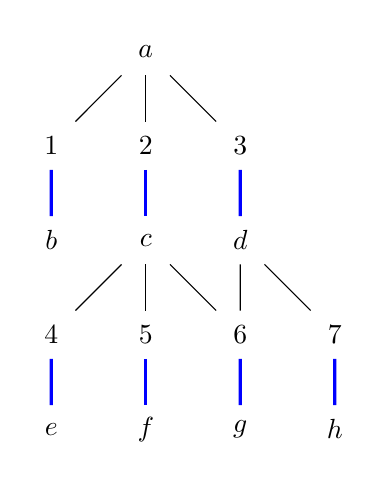
\begin{tikzpicture}[scale=1.2]
      \node (a) at (0,4) {$a$};
      \node (b) at (-1,2) {$b$};
      \node (c) at (0,2) {$c$};
      \node (d) at (1,2) {$d$};
      \node (e) at (-1,0) {$e$};
      \node (f) at (0,0) {$f$};
      \node (g) at (1,0) {$g$};
      \node (h) at (2,0) {$h$};
      \node (1) at (-1,3) {$1$};
      \node (2) at (0,3) {$2$};
      \node (3) at (1,3) {$3$};
      \node (4) at (-1,1) {$4$};
      \node (5) at (0,1) {$5$};
      \node (6) at (1,1) {$6$};
      \node (7) at (2,1) {$7$};

\foreach \a/\b in {a/1,a/2,a/3,c/4,c/5,c/6,d/6,d/7}
  \draw (\a) -- (\b);
\foreach \a/\b in {1/b,2/c,3/d,4/e,5/f,6/g,7/h}
  \draw[blue,very thick] (\a) -- (\b);
    \end{tikzpicture}
\end{document}
